\section{Zarządzanie}

Zarządzanie – ogólny zakres działań, procesów i decyzji, których zastosowanie w odniesieniu do zasobów, osób, kapitału lub organizacji ma zapewnić warunki do efektywnego ich funkcjonowania prowadzącego do osiągnięcia postawionych celów. \cite{French2010, Shotton1999, Shotton1989} 

\[
\sqrt{x^2+1}
\]

Od początku XX wieku, odkąd zarządzanie próbowano oprzeć na naukowych podstawach, aż do lat 60. XX wieku zarządzanie pojmowane było jako działanie kierownicze, obejmujące następujące sekwencje postępowania: planowanie, organizowanie, decydowanie, motywowanie i kontrolowanie, nazywane klasycznymi funkcjami zarządzania. \cite[123--126]{Lassen2006}

Klasyczne funkcje zarządzania wyróżnił pierwszy „klasyk” zarządzania Henri Fayol. Jednakże paradygmat zarządzania zmienił się od tego czasu radykalnie, więc warto powrócić do starszej, bardziej ogólnej definicji \textcite[610]{Porter1981} twierdz: zarządzanie to sztuka bądź praktyka rozumnego stosowania środków dla osiągnięcia wyznaczonych celów. \cite[25-28]{klimczak2007effect}

\subsection{Zarządzanie w gospodarce}

W odniesieniu do organizacji gospodarczych zamiast słowa zarządzanie używa się czasem terminu administracja biznesu (ang. Business Administration). Zadanie administracji biznesu ujmuje krótkie określenie: „Administracja biznesu ma zapewnić, aby zostało zrobione to, co ma być zrobione”. Administracja biznesu jest dyscypliną akademicką, a szereg uniwersytetów i szkół biznesu nadaje stopień magistra z tej dyscypliny (Master of Business Administration, w skrócie MBA). \cite{Lassen2006}

\begin{figure}[!ht]
	\centering
	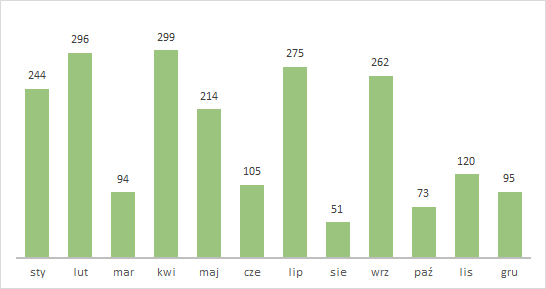
\includegraphics[width=\textwidth]{rozdzial1/wykres.png}
	\caption{{\bfseries Zmiana wartości w czasie}
	\\ \footnotesize{Źródło: \protect\cite{Shotton1999}}}
	\label{fig:wykres}
\end{figure}

\subsection{Zarządzanie w gospodarce}

W odniesieniu do organizacji gospodarczych zamiast słowa zarządzanie używa się czasem terminu administracja biznesu (ang. Business Administration). Zadanie administracji biznesu ujmuje krótkie określenie: „Administracja biznesu ma zapewnić, aby zostało zrobione to, co ma być zrobione”. Administracja biznesu jest dyscypliną akademicką, a szereg uniwersytetów i szkół biznesu nadaje stopień magistra z tej dyscypliny (Master of Business Administration, w skrócie MBA). \cite{Lassen2006}